% Created by tikzDevice version 0.10.1 on 2016-07-24 17:54:38
% !TEX encoding = UTF-8 Unicode
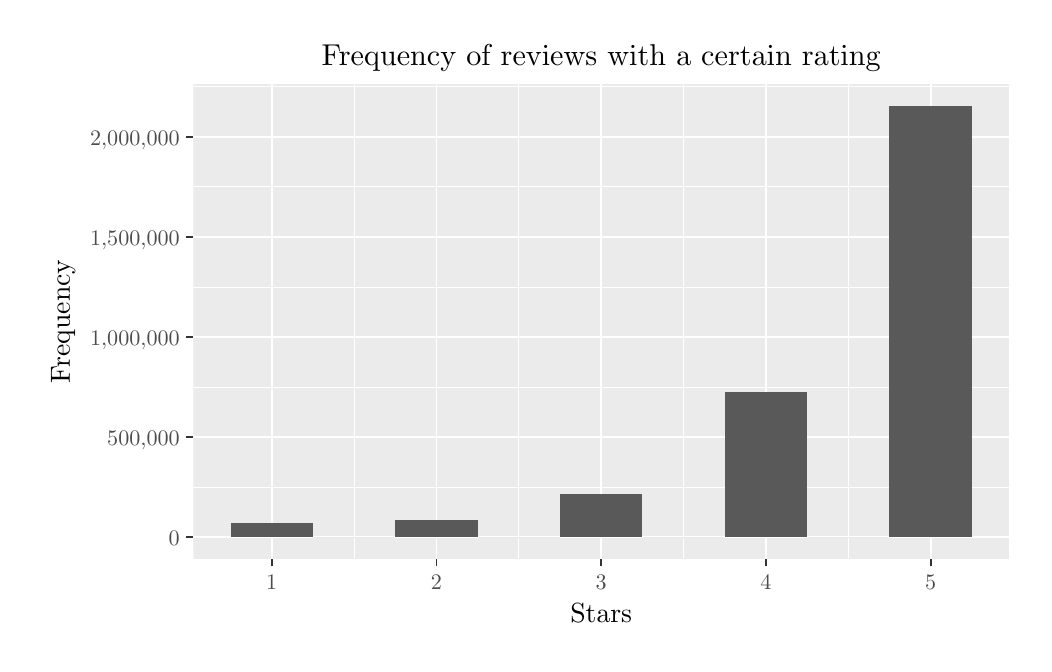
\begin{tikzpicture}[x=1pt,y=1pt]
\definecolor{fillColor}{RGB}{255,255,255}
\path[use as bounding box,fill=fillColor,fill opacity=0.00] (0,0) rectangle (360.07,222.54);
\begin{scope}
\path[clip] (  0.00,  0.00) rectangle (360.07,222.54);
\definecolor{drawColor}{RGB}{255,255,255}
\definecolor{fillColor}{RGB}{255,255,255}

\path[draw=drawColor,line width= 0.6pt,line join=round,line cap=round,fill=fillColor] (  0.00,  0.00) rectangle (360.07,222.54);
\end{scope}
\begin{scope}
\path[clip] ( 59.92, 30.62) rectangle (354.57,202.21);
\definecolor{fillColor}{gray}{0.92}

\path[fill=fillColor] ( 59.92, 30.62) rectangle (354.57,202.21);
\definecolor{drawColor}{RGB}{255,255,255}

\path[draw=drawColor,line width= 0.3pt,line join=round] ( 59.92, 56.51) --
	(354.57, 56.51);

\path[draw=drawColor,line width= 0.3pt,line join=round] ( 59.92, 92.67) --
	(354.57, 92.67);

\path[draw=drawColor,line width= 0.3pt,line join=round] ( 59.92,128.84) --
	(354.57,128.84);

\path[draw=drawColor,line width= 0.3pt,line join=round] ( 59.92,165.01) --
	(354.57,165.01);

\path[draw=drawColor,line width= 0.3pt,line join=round] ( 59.92,201.17) --
	(354.57,201.17);

\path[draw=drawColor,line width= 0.3pt,line join=round] (117.96, 30.62) --
	(117.96,202.21);

\path[draw=drawColor,line width= 0.3pt,line join=round] (177.48, 30.62) --
	(177.48,202.21);

\path[draw=drawColor,line width= 0.3pt,line join=round] (237.01, 30.62) --
	(237.01,202.21);

\path[draw=drawColor,line width= 0.3pt,line join=round] (296.53, 30.62) --
	(296.53,202.21);

\path[draw=drawColor,line width= 0.6pt,line join=round] ( 59.92, 38.42) --
	(354.57, 38.42);

\path[draw=drawColor,line width= 0.6pt,line join=round] ( 59.92, 74.59) --
	(354.57, 74.59);

\path[draw=drawColor,line width= 0.6pt,line join=round] ( 59.92,110.76) --
	(354.57,110.76);

\path[draw=drawColor,line width= 0.6pt,line join=round] ( 59.92,146.92) --
	(354.57,146.92);

\path[draw=drawColor,line width= 0.6pt,line join=round] ( 59.92,183.09) --
	(354.57,183.09);

\path[draw=drawColor,line width= 0.6pt,line join=round] ( 88.19, 30.62) --
	( 88.19,202.21);

\path[draw=drawColor,line width= 0.6pt,line join=round] (147.72, 30.62) --
	(147.72,202.21);

\path[draw=drawColor,line width= 0.6pt,line join=round] (207.25, 30.62) --
	(207.25,202.21);

\path[draw=drawColor,line width= 0.6pt,line join=round] (266.77, 30.62) --
	(266.77,202.21);

\path[draw=drawColor,line width= 0.6pt,line join=round] (326.30, 30.62) --
	(326.30,202.21);
\definecolor{fillColor}{gray}{0.35}

\path[fill=fillColor] ( 73.31, 38.42) rectangle (103.08, 43.59);

\path[fill=fillColor] (103.08, 38.42) rectangle (132.84, 38.42);

\path[fill=fillColor] (132.84, 38.42) rectangle (162.60, 44.71);

\path[fill=fillColor] (162.60, 38.42) rectangle (192.36, 38.42);

\path[fill=fillColor] (192.36, 38.42) rectangle (222.13, 53.87);

\path[fill=fillColor] (222.13, 38.42) rectangle (251.89, 38.42);

\path[fill=fillColor] (251.89, 38.42) rectangle (281.65, 90.85);

\path[fill=fillColor] (281.65, 38.42) rectangle (311.41, 38.42);

\path[fill=fillColor] (311.41, 38.42) rectangle (341.18,194.41);
\end{scope}
\begin{scope}
\path[clip] (  0.00,  0.00) rectangle (360.07,222.54);
\definecolor{drawColor}{gray}{0.30}

\node[text=drawColor,anchor=base east,inner sep=0pt, outer sep=0pt, scale=  0.80] at ( 54.97, 35.41) {0};

\node[text=drawColor,anchor=base east,inner sep=0pt, outer sep=0pt, scale=  0.80] at ( 54.97, 71.57) {500,000};

\node[text=drawColor,anchor=base east,inner sep=0pt, outer sep=0pt, scale=  0.80] at ( 54.97,107.74) {1,000,000};

\node[text=drawColor,anchor=base east,inner sep=0pt, outer sep=0pt, scale=  0.80] at ( 54.97,143.91) {1,500,000};

\node[text=drawColor,anchor=base east,inner sep=0pt, outer sep=0pt, scale=  0.80] at ( 54.97,180.07) {2,000,000};
\end{scope}
\begin{scope}
\path[clip] (  0.00,  0.00) rectangle (360.07,222.54);
\definecolor{drawColor}{gray}{0.20}

\path[draw=drawColor,line width= 0.6pt,line join=round] ( 57.17, 38.42) --
	( 59.92, 38.42);

\path[draw=drawColor,line width= 0.6pt,line join=round] ( 57.17, 74.59) --
	( 59.92, 74.59);

\path[draw=drawColor,line width= 0.6pt,line join=round] ( 57.17,110.76) --
	( 59.92,110.76);

\path[draw=drawColor,line width= 0.6pt,line join=round] ( 57.17,146.92) --
	( 59.92,146.92);

\path[draw=drawColor,line width= 0.6pt,line join=round] ( 57.17,183.09) --
	( 59.92,183.09);
\end{scope}
\begin{scope}
\path[clip] (  0.00,  0.00) rectangle (360.07,222.54);
\definecolor{drawColor}{gray}{0.20}

\path[draw=drawColor,line width= 0.6pt,line join=round] ( 88.19, 27.87) --
	( 88.19, 30.62);

\path[draw=drawColor,line width= 0.6pt,line join=round] (147.72, 27.87) --
	(147.72, 30.62);

\path[draw=drawColor,line width= 0.6pt,line join=round] (207.25, 27.87) --
	(207.25, 30.62);

\path[draw=drawColor,line width= 0.6pt,line join=round] (266.77, 27.87) --
	(266.77, 30.62);

\path[draw=drawColor,line width= 0.6pt,line join=round] (326.30, 27.87) --
	(326.30, 30.62);
\end{scope}
\begin{scope}
\path[clip] (  0.00,  0.00) rectangle (360.07,222.54);
\definecolor{drawColor}{gray}{0.30}

\node[text=drawColor,anchor=base,inner sep=0pt, outer sep=0pt, scale=  0.80] at ( 88.19, 19.64) {1};

\node[text=drawColor,anchor=base,inner sep=0pt, outer sep=0pt, scale=  0.80] at (147.72, 19.64) {2};

\node[text=drawColor,anchor=base,inner sep=0pt, outer sep=0pt, scale=  0.80] at (207.25, 19.64) {3};

\node[text=drawColor,anchor=base,inner sep=0pt, outer sep=0pt, scale=  0.80] at (266.77, 19.64) {4};

\node[text=drawColor,anchor=base,inner sep=0pt, outer sep=0pt, scale=  0.80] at (326.30, 19.64) {5};
\end{scope}
\begin{scope}
\path[clip] (  0.00,  0.00) rectangle (360.07,222.54);
\definecolor{drawColor}{RGB}{0,0,0}

\node[text=drawColor,anchor=base,inner sep=0pt, outer sep=0pt, scale=  1.00] at (207.25,  7.70) {Stars};
\end{scope}
\begin{scope}
\path[clip] (  0.00,  0.00) rectangle (360.07,222.54);
\definecolor{drawColor}{RGB}{0,0,0}

\node[text=drawColor,rotate= 90.00,anchor=base,inner sep=0pt, outer sep=0pt, scale=  1.00] at ( 15.24,116.42) {Frequency};
\end{scope}
\begin{scope}
\path[clip] (  0.00,  0.00) rectangle (360.07,222.54);
\definecolor{drawColor}{RGB}{0,0,0}

\node[text=drawColor,anchor=base,inner sep=0pt, outer sep=0pt, scale=  1.09] at (207.25,208.81) {Frequency of reviews with a certain rating};
\end{scope}
\end{tikzpicture}
